\documentclass[a4paper,11pt]{article}[24.3.2010]
\usepackage[left=2cm,top=3cm,text={17cm, 24cm}]{geometry}
\usepackage{amsthm}
\usepackage{times}
\usepackage{amsfonts}
\usepackage{amsmath}
\usepackage{graphics}
\usepackage{picture}
\usepackage{eurosym}
\usepackage{lastpage}
\usepackage[czech]{babel}
\usepackage[utf8]{inputenc}
\usepackage{fancyhdr}
\pagestyle{fancy}
\newcommand\myuv[1]{\quotedblbase #1\textquotedblleft}
\author{Jan Vybíral\\xvybir05@stud.fit.vutbr.cz}
\title{Typografie a publikování -- 1. projekt}
\date{}
\cfoot{\thepage\//\pageref{LastPage}}
\rhead{\textbf{Jan Vybíral, XVYBIR05}}

 
\begin{document}





\begin{enumerate}
  \item Uvažte jazyk $L_{1}=\{a^i b^j c^k \mid (i = 2j \lor j = 3k) \wedge i,j,k \geq 0\}$.
  \renewcommand{\theenumi}{\alph{enumi}}
  \begin{enumerate}
    \item Sestavte gramatiku $G_{1}$ takovou, že $L(G_{1}) = L_{1}$.\\\\    
      $G_{1}=(\{S,X,Y,U,V\},\{a,b,c\},P,S)$ s pravidly:\\
    \begin{eqnarray*}
      S&\rightarrow&X \mid Y \mid XU \mid VY\\
      X&\rightarrow&aaXb \mid \epsilon\\
      Y&\rightarrow&bbbYc\mid \epsilon\\
      U&\rightarrow&Uc\mid \epsilon\\
      V&\rightarrow&aV\mid \epsilon\\
    \end{eqnarray*}
    \item Jakého typu (dle Chomského hierarchie jazyků) je $G_{1}$ a jakého typu je $L_{1}$? Mohou se tyto typy obecně lišit? Svoje tvrzení zdůvodněte (formální důkaz není požadován).
    \begin{itemize}
        \item $G_{1}$ je typu 2 (bezkontextová gramatika), protože se na levých stranách jejích přepisovacích pravidel vyskytuje vždy jen jeden nonterminální symbol a nic dalšího a zároveň se na některých pravých stranách vyskytují pouze nonterminály.
        \item $L_{1}$ je typu 2, protože gramatika $G_{1}$, která ho generuje, je typu 2, a zároveň nemůže být generován gramatikou typu 3.
        \item  Platí, že $\mathcal{L}_{3} \subseteq \mathcal{L}_{2} \subseteq \mathcal{L}_{1} \subseteq \mathcal{L}_{0}$, kde $\mathcal{L}_{i}$ značí třídu všech jazyků typu $i$. Tudíž gramatika ${G}_{i}$ typu $i$ může generovat jazyk třídy $\mathcal{L}_{i}$ nebo jazyk některé konkrétnější třídy $\mathcal{L}_{j>i}$. Gramatika a jazyk, který generuje, mohou tedy být obecně jiného typu.\\
    \end{itemize}
  \end{enumerate}
  \renewcommand{\theenumi}{\arabic{enumi}}
  \item Uvažte regulární výraz  $r=(abc+\epsilon)^*a^*b$.
  \renewcommand{\theenumi}{\alph{enumi}}
  \begin{enumerate}
    \item Převeďte $r$ algoritmicky na redukovaný deterministický konečný automat $M$ (tj. RV $\rightarrow$ RKA $\rightarrow$ DKA $\rightarrow$ redukovaný DKA), přijímající jazyk popsaný výrazem $r$.
    \begin{itemize}
        \item Převod regulárního výrazu $r$ na rozšířený konečný automat.
        \item Rozklad regulárního výrazu vyjádříme stromem:
        \begin{figure}[h!]
        \begin{center}
        \scalebox{0.4}{
        \includegraphics{img/tree.png}
        }
        \end{center}
        \end{figure}
        \newpage

        \item Regulárnímu výrazu $r_{1}=a$ přísluší konečný automat $M_{1}$:
        \begin{figure}[h!]
        \begin{center}
        \scalebox{0.5}{
        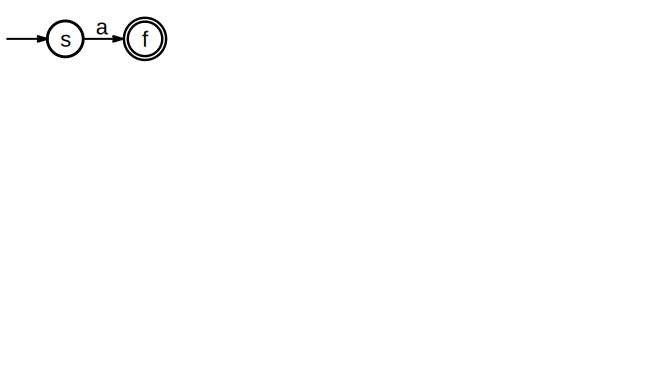
\includegraphics{img/a.png}
        }
        \end{center}
        \end{figure}
        \item Regulárnímu výrazu $r_{2}=b$ přísluší konečný automat $M_{2}$: 
        \begin{figure}[h!]
        \begin{center}
        \scalebox{0.5}{
        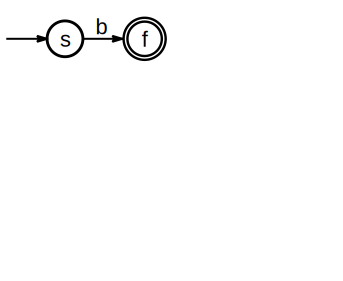
\includegraphics{img/b.png}
        }
        \end{center}
        \end{figure}
        \item Regulárnímu výrazu $r_{3}=ab$ přísluší konečný automat $M_{3}$:
        \begin{figure}[h!]
        \begin{center}
        \scalebox{0.5}{
        \includegraphics{img/ab.png}
        }
        \end{center}
        \end{figure}
        \item Regulárnímu výrazu $r_{4}=c$ přísluší konečný automat $M_{4}$:
        \begin{figure}[h!]
        \begin{center}
        \scalebox{0.5}{
        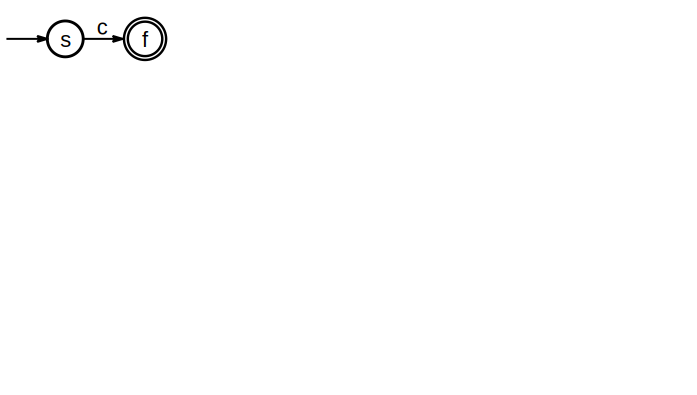
\includegraphics{img/c.png}
        }
        \end{center}
        \end{figure}
        \item Regulárnímu výrazu $r_{5}=abc$ přísluší konečný automat $M_{5}$:
        \begin{figure}[h!]
        \begin{center}
        \scalebox{0.5}{
        \includegraphics{img/abc.png}
        }
        \end{center}
        \end{figure}
        \item Regulárnímu výrazu $r_{6}=\epsilon$ přísluší konečný automat $M_{6}$: 
        \begin{figure}[h!]
        \begin{center}
        \scalebox{0.5}{
        \includegraphics{img/eps.png}
        }
        \end{center}
        \end{figure}
        \item Regulárnímu výrazu $r_{7}=abc+\epsilon$ přísluší konečný automat $M_{7}$.
        \begin{figure}[h!]
        \begin{center}
        \scalebox{0.5}{
        \includegraphics{img/abcpluseps.png}
        }
        \end{center}
        \end{figure}
        \item Regulárnímu výrazu $r_{8}=(abc+\epsilon)$ přísluší konečný automat $M_{7}$.
        \newpage

        \item Regulárnímu výrazu $r_{9}=(abc+\epsilon)^*$ přísluší konečný automat $M_{9}$:
        \begin{figure}[h!]
        \begin{center}
        \scalebox{0.5}{
        \includegraphics{img/abcplusepsh.png}
        }
        \end{center}
        \end{figure}
        \item Regulárnímu výrazu $r_{10}=r_{1}=a$ přísluší konečný automat $M_{1}$. 
        \item Regulárnímu výrazu $r_{11}=a^*$ přísluší konečný automat $M_{11}$:
        \begin{figure}[h!]
        \begin{center}
        \scalebox{0.5}{
        \includegraphics{img/ah.png}
        }
        \end{center}
        \end{figure}
        \item Regulárnímu výrazu $r_{12}=r_{2}=b$ přísluší konečný automat $M_{2}$.
        \item Regulárnímu výrazu $r_{13}=a^*b$ přísluší konečný automat $M_{13}$:
        \begin{figure}[h!]
        \begin{center}
        \scalebox{0.5}{
        \includegraphics{img/ahb.png}
        }
        \end{center}
        \end{figure}
        

        \item Výslednému regulárnímu výrazu  $r=(abc+\epsilon)^*a^*b$ přísluší rozšířený konečný automat $M_{R}$:
        \begin{figure}[h!]
        \begin{center}
        \scalebox{0.5}{
        \includegraphics{img/final.png}
        }
        \end{center}
        \end{figure}
\newpage
        \item Převedeme rozšířený konečný automat $M_{R}$ na úplný deterministický konečný automat\\ $M_{D} = (Q,\{a,b,c\},\delta,A,F)$.\\
        \item Počáteční stav $M_{D}$ = $\epsilon$-uzávěr$(s)=\{s,1,2,6,7,8,9,10,12\} = A$.
        \item $\delta(A,a)=\epsilon$-uzávěr$(\{3,11\})=\{3,10,11,12\}=B$.
        \item $\delta(A,b)=\epsilon$-uzávěr$(\{f\})=\{f\}=C$.
        \item $\delta(A,c)=\epsilon$-uzávěr$(\emptyset)=\emptyset=D$.
        \item $\delta(B,a)=\epsilon$-uzávěr$(\{11\})=\{10,11,12\}=E$.
        \item $\delta(B,b)=\epsilon$-uzávěr$(\{4,f\})=\{4,f\}=G$.
        \item $\delta(B,c)=\epsilon$-uzávěr$(\emptyset)=\emptyset=D$.
        \item $\delta(C,a)=\epsilon$-uzávěr$(\emptyset)=\emptyset=D$.
        \item $\delta(C,b)=\epsilon$-uzávěr$(\emptyset)=\emptyset=D$.
        \item $\delta(C,c)=\epsilon$-uzávěr$(\emptyset)=\emptyset=D$.
        \item $\delta(D,a)=\epsilon$-uzávěr$(\emptyset)=\emptyset=D$.
        \item $\delta(D,b)=\epsilon$-uzávěr$(\emptyset)=\emptyset=D$.
        \item $\delta(D,c)=\epsilon$-uzávěr$(\emptyset)=\emptyset=D$.
        \item $\delta(E,a)=\epsilon$-uzávěr$(\{11\})=\{10,11,12\}=E$.
        \item $\delta(E,b)=\epsilon$-uzávěr$(\{f\})=\{f\}=C$.
        \item $\delta(E,c)=\epsilon$-uzávěr$(\emptyset)=\emptyset=D$.
        \item $\delta(G,a)=\epsilon$-uzávěr$(\emptyset)=\emptyset=D$.
        \item $\delta(G,b)=\epsilon$-uzávěr$(\emptyset)=\emptyset=D$.
        \item $\delta(G,c)=\epsilon$-uzávěr$(\{5\})=\{1,2,5,6,7,8,9,10,12\}=H$.
        \item $\delta(H,a)=\epsilon$-uzávěr$(\{3,11\})=\{3,10,11,12\}=B$.
        \item $\delta(H,b)=\epsilon$-uzávěr$(\{f\})=\{f\}=C$.
        \item $\delta(H,c)=\epsilon$-uzávěr$(\emptyset)=\emptyset=D$.
        \item Výsledná množina stavů $Q=\{A,B,C,D,E,G,H\}$
        \item Množina koncových stavů $F=\{C,G\}$


        \item Výsledný úplný deterministický konečný automat $M_{D}$:
        \begin{figure}[h!]
        \begin{center}
        \scalebox{0.5}{
        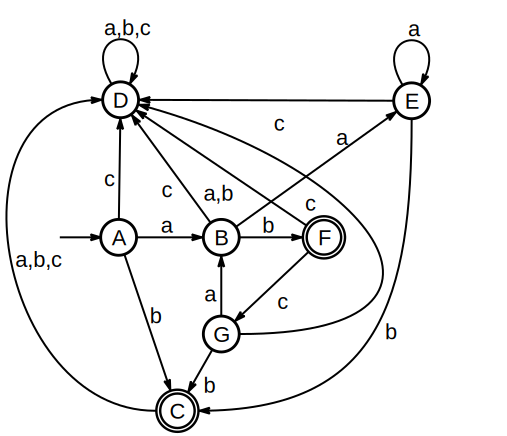
\includegraphics{img/dka2.png}
        }
        \end{center}
        \end{figure}
 \newpage
        \item Převod úplného deterministického konečného automatu  $M_{D}$ na výsledný redukovaný deterministický konečný automat  $M$.
        \item $M_{D}$ neobsahuje nedostupné stavy. Odstraníme nerozlišitelné stavy:
        
        \begin{table}[ht]
        \begin{center}
        \begin{tabular}{ c  c | c  c  c } 
        $\overset{0}{\equiv}$ & $\delta$ & $a$ & $b$ & $c$ \\ 
        \hline
        $I:$ & $C$ & $D_{II}$ & $D_{II}$ & $D_{II}$ \\ 
        & $G$ & $D_{II}$ & $D_{II}$ & $H_{II}$ \\
        \hline
        $II:$ & $A$ & $B_{II}$ & $C_{I}$ & $D_{II}$ \\ 
        & $B$ & $E_{II}$ & $G_{I}$ & $D_{II}$ \\
        & $D$ & $D_{II}$ & $D_{II}$ & $D_{II}$ \\
        & $E$ & $E_{II}$ & $C_{I}$ & $D_{II}$ \\
        & $H$ & $B_{II}$ & $C_{I}$ & $D_{II}$ \\
        \end{tabular}
        \quad
        \begin{tabular}{ c  c | c  c  c } 
        $\overset{1}{\equiv}$ & $\delta$ & $a$ & $b$ & $c$ \\ 
        \hline
        $I:$ & $C$ & $D_{III}$ & $D_{III}$ & $D_{III}$ \\ 
        & $G$ & $D_{III}$ & $D_{III}$ & $H_{II}$ \\
        \hline
        $II:$ & $A$ & $B_{II}$ & $C_{I}$ & $D_{III}$ \\ 
        & $B$ & $E_{II}$ & $G_{I}$ & $D_{III}$ \\
        & $E$ & $E_{II}$ & $C_{I}$ & $D_{III}$ \\
        & $H$ & $B_{II}$ & $C_{I}$ & $D_{III}$ \\
        \hline
        $III:$ & $D$ & $D_{III}$ & $D_{III}$ & $D_{III}$ \\
        \end{tabular}
        \end{center}
        \end{table}

        \begin{table}[ht]
        \begin{center}
        \begin{tabular}{ c  c | c  c  c } 
        $\overset{2}{\equiv}$ & $\delta$ & $a$ & $b$ & $c$ \\ 
        \hline
        $I:$ & $C$ & $D_{IV}$ & $D_{IV}$ & $D_{IV}$ \\ 
        \hline
        $II:$ & $G$ & $D_{IV}$ & $D_{IV}$ & $H_{III}$ \\ 
        \hline
        $III:$ & $A$ & $B_{III}$ & $C_{I}$ & $D_{IV}$ \\ 
        & $B$ & $E_{III}$ & $G_{II}$ & $D_{IV}$ \\
        & $E$ & $E_{III}$ & $C_{I}$ & $D_{IV}$ \\
        & $H$ & $B_{III}$ & $C_{I}$ & $D_{IV}$ \\
        \hline
        $IV:$ & $D$ & $D_{IV}$ & $D_{IV}$ & $D_{IV}$ \\
        \end{tabular}
        \quad
        \begin{tabular}{ c  c | c  c  c } 
        $\overset{3}{\equiv}$ & $\delta$ & $a$ & $b$ & $c$ \\ 
        \hline
        $I:$ & $C$ & $D_{V}$ & $D_{V}$ & $D_{V}$ \\ 
        \hline
        $II:$ & $G$ & $D_{V}$ & $D_{V}$ & $H_{III}$ \\ 
        \hline
        $III:$ & $A$ & $B_{IV}$ & $C_{I}$ & $D_{V}$ \\ 
        & $E$ & $E_{III}$ & $C_{I}$ & $D_{V}$ \\
        & $H$ & $B_{IV}$ & $C_{I}$ & $D_{V}$ \\
        \hline
        $IV:$ & $B$ & $E_{III}$ & $G_{II}$ & $D_{V}$ \\
        \hline
        $V:$ & $D$ & $D_{V}$ & $D_{V}$ & $D_{V}$ \\
        \end{tabular}
        \end{center}
        \end{table}


        \begin{table}[ht]
        \begin{center}
        \begin{tabular}{ c  c | c  c  c } 
        $\overset{3}{\equiv}$ & $\delta$ & $a$ & $b$ & $c$ \\ 
        \hline
        $I:$ & $C$ & $D_{VI}$ & $D_{VI}$ & $D_{VI}$ \\ 
        \hline
        $II:$ & $G$ & $D_{VI}$ & $D_{VI}$ & $H_{III}$ \\ 
        \hline
        $III:$ & $A$ & $B_{V}$ & $C_{I}$ & $D_{VI}$ \\ 
        & $H$ & $B_{V}$ & $C_{I}$ & $D_{VI}$ \\
        \hline
        $IV:$ & $E$ & $E_{IV}$ & $C_{I}$ & $D_{VI}$ \\
        \hline
        $V:$ & $B$ & $E_{IV}$ & $G_{II}$ & $D_{VI}$ \\
        \hline
        $VI:$ & $D$ & $D_{VI}$ & $D_{VI}$ & $D_{VI}$ \\
        \end{tabular}
        \end{center}
        \end{table}

        \item Výsledný redukovaný deterministický konečný automat $M$:
        \begin{figure}[h!]
        \begin{center}
        \scalebox{0.43}{
        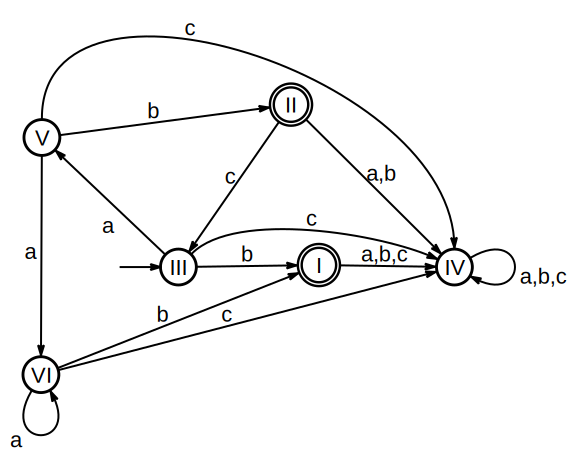
\includegraphics{img/result.png}
        }
        \end{center}
        \end{figure}
    \end{itemize}
\newpage

   \item Pro jazyk $L(M)$ určete počet tříd ekvivalence relace $\sim_{L}$ (viz. Myhill-Nerodova věta) a vypište tyto třídy. Jednotlivé třídy můžete popsat například konečným automatem, který akceptuje všechna slova patřící do dané třídy.\\\\
   Celkem 6 tříd:\\
   


\begin{figure}[htbp]
 \begin{minipage}{0.5\linewidth}
  \centering
  \scalebox{0.3}{
   \includegraphics{img/ca.png}
   }
  \caption{$L^{-1}(I)$}
 \end{minipage}%
 \begin{minipage}{0.5\linewidth}
  \centering
  \scalebox{0.3}{
   \includegraphics{img/cb.png}
   }
  \caption{$L^{-1}(II)$}
 \end{minipage}
\end{figure} 

\begin{figure}[htbp]
 \begin{minipage}{0.5\linewidth}
  \centering
  \scalebox{0.4}{
   \includegraphics{img/cc.png}
   }
  \caption{$L^{-1}(III)$}
 \end{minipage}%
 \begin{minipage}{0.5\linewidth}
  \centering
  \scalebox{0.4}{
   \includegraphics{img/qf.png}
   }
  \caption{$L^{-1}(IV)$}
 \end{minipage}
\end{figure} 

\begin{figure}[htbp]
 \begin{minipage}{0.5\linewidth}
  \centering
  \scalebox{0.3}{
   \includegraphics{img/ce.png}
   }
  \caption{$L^{-1}(V)$}
 \end{minipage}%
 \begin{minipage}{0.5\linewidth}
  \centering
  \scalebox{0.3}{
   \includegraphics{img/cd.png}
   }
  \caption{$L^{-1}(VI)$}
 \end{minipage}
\end{figure} 



   \newpage

   
  \end{enumerate}
  \renewcommand{\theenumi}{\arabic{enumi}}
\newpage

  \item Uvažte NKA $M_{3}$ nad abecedou $\Sigma=\{a,b,c\}$ z obrázku:
  \begin{figure}[h!]
  \begin{center}
  \scalebox{0.5}{
  \includegraphics{img/3.png}
  }
  \end{center}
  \caption{NKA $M_{3}$}
  \end{figure} \\
  Řešením rovnic nad regulárními výrazy sestavte k tomuto automatu ekvivalentní regulární výraz.\\\\
  Sestavíme soustavu rovnic nad regulárními výrazy pro $M_{3}$: \\\\
  $X_{1}=aX_{2}$ \\
  $X_{2}=bX_{3}+cX_{1}$ \\
  $X_{3}=\epsilon+aX_{2}+bX_{1}$ \\\\
  Regulárnímu výrazu ekvivalentnímu automatu $M_{3}$ odpovídá řešení této soustavy pro $X_{1}$.\\\\
  Dosadíme do třetí rovnice za $aX_{2}$ podle první rovnice:\\\\
  $X_{3}=\epsilon+X_{1}+bX_{1}$\\\\
  Dosadíme výsledek do druhé rovnice za $X_{3}$:\\\\
  $X_{2}=b(\epsilon+X_{1}+bX_{1})+cX_{1}=b+bX_{1}+bbX_{1}+cX_{1}$\\\\
  Dosadíme výsledek do první rovnice za $X_{2}$:\\\\
  $X_{1}=a(b+bX_{1}+bbX_{1}+cX_{1})=ab+abX_{1}+abbX_{1}+acX_{1}=(ab+abb+ac)X_{1}+ab$ \\\\
  Nejmenším pevným bodem rovnice nad regulárními výrazy ve tvaru $X=pX+q$ je $X=p^*q$, řešení pro $X_{1}$ a hledaný regulární výraz tedy je:\\\\
  $X_{1}=(ab+abb+ac)^*ab$\\

\newpage

  \item Mějme funkci $\Phi : \Sigma^* \rightarrow (\Sigma \cup \{\bullet\})^*$, kde $\bullet \notin \Sigma$, která každý třetí symbol ve slově nahradí symbolem $\bullet$. Formálně je $\Phi$ definována následujícím předpisem:
    \begin{itemize}
      \item $\Phi(\epsilon) = \epsilon$
      \item $\Phi(a_{1}) = a_{1}$, kde $a_{1} \in \Sigma$
      \item $\Phi(a_{1}a_{2}) = a_{1}a_{2}$, kde $a_{1},a_{2} \in \Sigma$
      \item $\Phi(a_{1}a_{2}a_{3}u) = a_{1}a_{2}\bullet\Phi(u)$, kde $a_{1},a_{2},a_{3} \in \Sigma, u \in \Sigma^*$
    \end{itemize}
    Například: $\Phi(aaa) = aa\bullet, \Phi(abcde) = ab\bullet de, \Phi(abcdef) = ab\bullet de\bullet$\\\\
Navrhněte a formálně popište algoritmus, který má na vstupu konečný automat $M_{1}=(Q,\Sigma,\delta,q_{0},F)$ (může být nedeterministický), a jehož výstupem bude konečný automat $M_{2}$ takový, že $L(M_{2})=\{\Phi(w) \mid w \in L(M_{1})\}$.\\

{\bf Algoritmus:}\\\\
{\bf Vstup:} Konečný automat $M_{1}=(Q_{1},\Sigma_{1},\delta_{1},q_{01},F_{1})$ (může být i nedeterministický)\\\\
{\bf Výstup:} Konečný automat $M_{2}=(Q_{2},\Sigma_{2},\delta_{2},q_{02},F_{2})$ takový, že $L(M_{2})=\{\Phi(w) \mid w \in L(M_{1})\}$\\\\
{\bf Metoda:}
\begin{itemize}
\item Polož $Q=\{0, 1, 2\}$
\item Polož $Q_{2}= Q_{1} \times Q$
\item Polož $\Sigma_{2}= \Sigma_{1} \cup \{\bullet\}$
\item Zkonstruuj $\delta_{2} : Q_{2} \times \Sigma_{2} \rightarrow 2^{Q_{2}}$ tak, že:\\
$\forall q_{1}, q_{2} \in Q_{1} \hspace{4pt} \forall q_{3}, q_{4} \in Q \hspace{4pt} \forall a \in \Sigma_{2}:\\ 
(q_{2}, q_{4}) \in \delta_{2}((q_{1}, q_{3}), a) \Leftrightarrow\\ 
(a \neq \bullet \wedge q_{2} \in \delta_{1}(q_{1}, a) \wedge ((q_{3}=0 \wedge q_{4}=1) \vee (q_{3}=1 \wedge q_{4}=2))) \vee\\
(a = \bullet \wedge \exists b \in \Sigma_{1} : q_{2} \in \delta_{1}(q_{1}, b) \wedge q_{3}=2 \wedge q_{4}=0)$
\item Polož $q_{02}= (q_{01}, 0)$
\item Polož $F_{2}= F_{1} \times Q$

\end{itemize}

\newpage

  \item Mějme jazyk $L=\{w\mid w \in \{a,b,c,d\}^{*} \wedge \#_{a}(w) = \#_{b}(w) \wedge \#_{c}(w) = \#_{d}(w)\}$, kde $\#_{x}(w)$ je počet symbolů $x$ ve slově $w$. Je jazyk $L$ regulární? Dokažte nebo vyvraťte.\\

Jazyk $L$ je nekonečný. Předpokládejme, že jazyk $L$ je regulární. Pak podle Pumping lemma pro regulární jazyky platí:\\
$\exists k > 0: \forall w \in L: |w| \geq k \Rightarrow \exists x,y,z \in \Sigma^{*}: w = xyz \wedge |y| > 0 \wedge |xy| \leq k \wedge \forall i \geq 0: xy^{i}z \in L$\\

Uvažme libovolné $k > 0$ takové, že:\\
$\forall w \in L: |w| \geq k \Rightarrow \exists x,y,z \in \Sigma^{*}: w = xyz \wedge |y| > 0 \wedge |xy| \leq k \wedge \forall i \geq 0: xy^{i}z \in L$\\

Zvolme $w=a^{k}b^{k} \in L$, $|w| = 2k > k$ a tedy z výše uvedeného:\\
$\exists x,y,z \in \Sigma^{*}: w=a^{k}b^{k} = xyz \wedge |y| > 0 \wedge |xy| \leq k \wedge \forall i \geq 0: xy^{i}z \in L$\\

Uvažme libovolné $x,y,z \in \Sigma^{*}$ takové, že:\\
$w = a^{k}b^{k} = xyz \wedge |y| > 0 \wedge |xy| \leq k \wedge \forall i \geq 0: xy^{i}z \in L$\\

Zvolme $i=2k> 0$, tedy:\\
$w = a^{k}b^{k} = xyz \wedge |y| > 0 \wedge |xy| \leq k \wedge v = xy^{2k}z \in L$\\

Z toho je zřejmé, že řetězec $xy$ může obsahovat pouze symboly $a$, proto pro řetězec $v$ musí platit, že:\\
$\#_{a}(v) \geq 2k \wedge \#_{b}(v) = k$,\\

tudíž\\ 
$\#_{a}(v) > \#_{b}(v)$,\\

takže\\
$v = xy^{2k}z \notin L$,\\

což je SPOR. Jazyk L tudíž není regulární.\newpage


\item Dokažte, že pro každý regulární jazyk existuje jednoznačná gramatika (definice jednoznačné gramatiky - viz. slidy 4, strana 11).\\\\
Podle definice \textbf{4.5} ze slidů 4 je jednoznačná gramatika taková gramatika, ve které existuje pro každou větu, kterou v ní lze vygenerovat, jen jeden derivační strom s koncovými uzly tvořícími tuto větu.\\\\
Dále podle studijní opory platí:\\
\begin{itemize}
\item Každý regulární jazyk lze vyjádřit ekvivalentním regulárním výrazem.\\
\item Každý regulární výraz lze převést na ekvivalentní deterministický konečný automat (např. algoritmy \textbf{3.7} a \textbf{3.6} ve studijní opoře).\\
\item Podle důkazu věty \textbf{3.7} ve studijní opoře lze každý deterministický konečný automat $M=(Q, \Sigma, \delta, q_{0}, F)$ vyjádřit ekvivalentní gramatikou $G=(Q, \Sigma, P, q_{0})$ typu 3 s pravidly definovanými takto:\\
\begin{enumerate}
      \item Je-li $\delta(q,a)=r$, pak P obsahuje pravidlo $q\rightarrow ar$
      \item Je-li $p \in F$, pak P obsahuje pravidlo $p\rightarrow \epsilon$\\
\end{enumerate}
kde $q,r,p \in Q$, $a \in \Sigma$\\
\item Z bodu (a) plyne, že $G$ nemůže obsahovat žádná dvě pravidla tvaru:
\begin{eqnarray*}
      q&\rightarrow&ar_{1}\\
      q&\rightarrow&ar_{2}\\
\end{eqnarray*}
kde $q,r_{1},r_{2},p \in Q$, $a \in \Sigma$, taková, že $r_{1}\neq r_{2}$\\
\item Z toho je zřejmé, že v gramatice $G$ nemůžou existovat dvě různé posloupnosti přímých derivací začínajících počátečním neterminálem, na jejichž konci by byla tatáž věta.  Tím pádem v gramatice $G$ musí pro každou větu, kterou v ní lze vygenerovat, existovat pouze jeden derivační strom s koncovými uzly tvořícími tuto větu. Takto sestavená gramatika $G$ musí tudíž vždy být jednoznačná. \\
\item Z předchozích bodů plyne, že každý regulární jazyk lze převést na ekvivalentní jednoznačnou gramatiku, a tudíž je dokázáno, že pro každý regulární jazyk existuje jednoznačná gramatika.
\end{itemize}




 

\end{enumerate}






\end{document}